%%% Pfitzner
\begin{frame}[t]
    
    \begin{block}{\af}
        \cit{
            Autorka nie sformułowała tezy rozprawy, co wynika ze specyfiki pracy, natomiast celem praktycznym było opracowanie takiego rozwiązania konstrukcyjnego przedwzmacniacza, aby umożliwić skuteczną realizację zintegrowanego narzędzia do badań mózgu przez zespół Katedry Oddziaływań i Detekcji Cząstek AGH.
        }
    \end{block}

    \begin{block}{\dk}
        \cit{
            W przypadku przedstawionej pracy Autorka precyzyjnie przedstawiła główny cel pracy oraz wyszczególniła kolejny etapy pracy prowadzące do realizacji celu głównego.
            Niestety w pracy nie zauważyłem wyszczególnionych tez pracy. 
            \high{
                Jakie są zatem cele pracy? Czy tezy pracy zostały udowodnione?
            }}
    \end{block}
    Tezy prace są tożsame z celem pracy i explicite nie zostały sformułowane w ramach odrębnych stwierdzeń.
    Rozumiem, że byłoby to przydatne podczas czytania.%, chociaż uważałam to w momencie za nienaturalne z wyżej wymienionego powodu.

\end{frame}


\begin{frame}[t]
    \vspace{-1em}

    \begin{block}{\dk}
        \cit{
            {\renewcommand\normalsize{\small}%
            \normalsize
            Struktura rozprawy jest logiczna, jednak w pracy występuje pewna (moim zdaniem stanowczo zbyt liczna) liczba uchybień edycyjnych (tekstowych, językowych), np. forma gramatyczna, powtórzenia, brak przedimków lub słów itp.
            }
        }
    \end{block}
    \vspace{-1em}

    \begin{block}{\af}
        \cit{
            {\renewcommand\normalsize{\small}%
            \normalsize
            W tekście pracy jest relatywnie dużo literówek, występują też drobne błędy gramatyczne, co świadczy prawdopodobnie o nadmiernie pospiesznym finalizowaniu rozprawy. 
            Innych niedociągnięć jest niewiele, np.: na rysunkach 3.13 i 3.14 na osi odciętych skala częstotliwości obejmuje zakres od 0.1 Hz do 100 Hz, podczas gdy w podpisie podano pasmo 1 Hz -- 10 kHz. 
            Ponadto tabela 4.3 jest wadliwie zbudowana i bez dodatkowego opisu nieczytelna.
            }
        }
    \end{block}

    \begin{columns}

        \column{.35\textwidth}
        \vspace{-1.5em}
        \begin{figure}[H]
            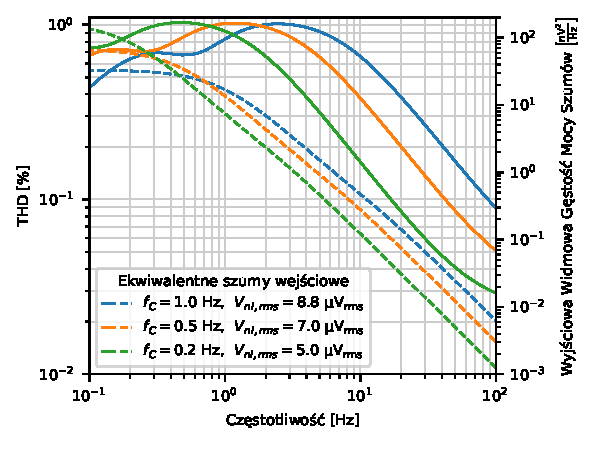
\includegraphics[scale = 0.45]{Figures/thd_f_C.pdf}
        \end{figure}
    
        \column{.65\textwidth}

        {\renewcommand\normalsize{\small}%
        \normalsize
        Zależność współczynnika THD od częstotliwości oraz rozkłady PSD na wyjściu dla różnych ustawień częstotliwości granicznej przy stałej wartości $C_{in} = \SI{4}{\pico\farad}$ i wzmocnieniu $\SI{20}{\frac{\volt}{\volt}}$.
        Amplituda sygnału: $\SI{10}{\milli\volt_{pp}}$.
        Wartości napięcia $V_{gs} $ były ustawione dla każdej symulacji niezależnie, aby uzyskać wymagane wartości dolnej częstotliwości granicznej.  
        Na wykresie \textbf{w legendzie} zostały \textbf{podane} ekwiwalentne szumy wejściowe w paśmie $\SI{1}{\hertz}$ -- $\SI{10}{\kilo\hertz}$ dla poszczególnych rozwiązań.
        }
    
    \end{columns}
\end{frame}

\begin{frame}[t]
    
Ekwiwalentne szumy wejściowe dla różnych parametrów przedwzmacniacza [$\SI{}{\micro\volt_{rms}}$]. 
Dla każdego prądu polaryzującego i częstotliwości granicznej przedstawiono ekwiwalentne szumy wejściowe dla dwóch zakresów częstotliwości: 1 -- 300 Hz (pasmo LFP) i 300 Hz -- 10 kHz (pasmo AP).
\begin{table}
    \centering

    \label{table:noseLFP_AP_ibias}
    \begin{tabular}{c||l||l||l||l||l||l}
    \diagbox{\begin{tabular}[c]{@{}l@{}}Częstotliwość \\graniczna [Hz]\end{tabular}}{\begin{tabular}[c]{@{}l@{}}\textbf{\textbf{Prąd polaryzujący }}\\\textbf{\textbf{wzmacniacz }}\\\textbf{\textbf{[$\SI{}{\micro\ampere}$]}}\\\textbf{}\\\textbf{}\end{tabular}} & \multicolumn{2}{c||}{\textbf{2~}} & \multicolumn{2}{c||}{\textbf{\textbf{4~}}} & \multicolumn{2}{c}{\textbf{\textbf{6~}}}  \\ 
    \hhline{~|:=:t:=::=:t:=::=:t:=}
    \multicolumn{1}{l||}{}                                                                                                                                                                                                                                          & LFP  & AP                         & LFP  & AP                                  & LFP  & AP                                 \\ 
    \hhline{=::=::=::=::=::=::=}
    1,0                                                                                                                                                                                                                                                             & 9,16 & 6,18                       & 9,03 & 4,60                                & 9,02 & 3,93                               \\
    0,5                                                                                                                                                                                                                                                             & 7,49 & 6,15                       & 7,29 & 4,57                                & 7,26 & 3,90                               \\
    0,2                                                                                                                                                                                                                                                            & 5,66 & 6,13                       & 5,44 & 4,55                                & 5,41 & 3,87                              
    \end{tabular}
    \end{table}

        
\end{frame}

\begin{frame}[t]
    \vspace{-1em}
    \begin{block}{\af}
        \cit{
            {\renewcommand\normalsize{\small}%
            \normalsize
            Zwykle jednak wymagania projektowe formułowane są explicite w formie granicznych wartości istotnych parametrów, lecz takich na dla pracy nie określono. 
            W tej sytuacji pierwszorzędnego znaczenia nabiera porównanie wartości osiągniętych parametrów zaprojektowanego wzmacniacza z danymi dostępnymi z literatury. 
            Brak zestawienia porównawczego w formie tabeli budzi pewien niedosyt. 
            Wprawdzie standardowo w odniesieniu do zniekształceń harmonicznych wartość THD podawana jest zwykle dla częstotliwości 1 kHz, a nie w szerszym zakresie, to jednak takie zestawienie byłoby zasadne, uwzględniając zarówno ogólne stwierdzenia, jak i wartości innych parametrów.}
        }
    \end{block}
    {\renewcommand\normalsize{\small}%
\normalsize
Powodem, dla którego nie zostały podane sztywne wartości dotyczące systemu, wynika z tego, że celem projektu było zbadanie możliwości zbudowanie takiego wzmacniacza w wybranej technologii. Nie celowano w konkretny zestaw parametrów, ponieważ powierzchnia, moc i szumy są parametrami, które się wymieniają i optymalizacja jednego parametru pogarsza pozostałe parametry.
W trakcie opracowywania układu pamiętano jaki zakres parametrów jest wymagany, by nadawał się do rejestracji.
Zbudowano kilka struktur testowych umożliwiających eksplorowanie ograniczeń technologicznych pod kątem budowy odczytu dla wielokanałowej sondy. 

}
    
\end{frame}

%%% Komorowski

\begin{frame}[t]
    \begin{block}{\dk}
        \cit{
            Omówiono również inne koncepcje eliminacji składowej stałej: technikę wzmacniaczy z modulacją [...] oraz zastosowanie wzmacniacza o małym lub jednostkowym wzmocnieniu i przetwornika analogowo-cyfrowego o dużej rozdzielczości.
            Z uwagi na rosnącą popularność tego ostatniego rozwiązania w przypadku akwizycji sygnałów biologicznych i biomedycznych uważam, że ta część rozdziału powinna być bardziej szczegółowa. 
        }
    \end{block}

    Rozumiem, że w kontekście rosnącej popularności rozwiązań opartych o wzmacniacz o małym lub jednostkowym wzmocnieniu i przetwornik analogowo-cyfrowy ubogi fragment w rozdziale dotyczącym obecnego stanu wiedzy budzi niedosyt.
    Rozwiązania te jednak tyczą  się głównie zastosowań związanych z rejestracją sygnałów EEG. Układy  te charakteryzują się innymi wymaganiami dotyczącymi ilości kanałów pomiarowych, rozmiarów oraz technologii, w której są wykonywane.
    Dlatego zdecydowano się nie poszerzać pracy o ten aspekt, szczególnie że w przypadku systemów dedykowanych rejestracji mikroelektrodowej aplikowanych wewnątrz mózgu nie jest to kierunek wiodący.

\end{frame}

\begin{frame}[t]
    \begin{block}{\dk}
        \cit{
            W pracy występuje dość obszerna część medyczno-biologiczna służąca w zasadzie do uzasadnienia podziału sygnałów na dwie grupy LFP i AP o odpowiednich charakterystykach (pasmo i zakres amplitud).
            Materiał ciekawy i ważny z punktu widzenia pracy, ale być może mógłby być krótszy.
        }
    \end{block}
    Z jednej strony ten materiał mógłby być krótszy, ale z drugiej strony uwagi pana dr. hab. Buchnera sugerują, że powinien być bardziej rozbudowany.
\end{frame}

\begin{frame}[t]
    \begin{block}{\dk}
        \cit{
            Niektóre używane w pracy określenia moim zdaniem są nietypowe, głównie dotyczy to określenia "\high{układ odczytu}" zamiast wzmacniacz.
            [...]
            Podobnie użycie słowa "\high{zaadresowany}".
            Wyrażenie "\high{mniejsze multipleksery}" (str. 34) jest mało precyzyjne, a właściwie w użytym kontekście nieprawidłowe.
            Również definicja wyrażenia "\high{front-end}" (str. 35) budzi moje wątpliwości.
            Użycie wyrażenia "\high{może zostać drastycznie zmniejszona}" wydaje mi się również niezbyt fortunne.
            Autorka rozprawy dosyć często używa wyrażenia \high{offset wyjściowy}, moim zdaniem jednak poprawnie powinno się stosować wyrażenie offset napięcia wyjściowego.
        }
    \end{block}

    \begin{columns}
        \column{.3\textwidth}
        \vspace{-1em}
        \begin{figure}[H]
            \includegraphics[scale = 0.2]{ch2/afe.png}
        \end{figure}

        \column{.75\textwidth}
        {\renewcommand\normalsize{\small}%
        \normalsize
            Układ odczytu jest pojęciem szerszym aniżeli wzmacniacz, który jest częścią układu odczytowego. 
            Pojęcie może jest niefortunne i lepsze byłoby określenie \high{tor odczytu} opisując drogę sygnału. 
            Dodatkowo pojęcie \textit{Front End} jest powszechnie używane w kontekście struktur scalonych, opisując fragment toru odczytowego, który odpowiada za wstępne przetworzenie sygnału.
            Pojęcie mniejsze multipleksery jest niefortunne -- chodziło o multipleksery obejmujące mniejszą liczbę kanałów wejściowych. 
            Dzięki mniejszej liczbie kanałów można wykorzystywać niższe częstotliwości zegarów odpowiedzialnych za próbkowanie sygnału.
        }
    \end{columns}
    
\end{frame}



\begin{frame}[t]
    \begin{block}{\dk}
        \cit{
            \high{Wzmacniacz LNA występuje w każdym kanale, skąd następnie sygnał jest przesyłany poprzez MUX z podziałem czasu.
            Wadą tego rozwiązania jest to, że gdy liczba kanałów wzrasta, częstotliwość próbkowania ADC również wzrasta, co powoduje większy pobór mocy.} - Częstotliwość próbkowania powinna być zależna od właściwości próbkowanego (rejestrowanego) sygnału, a nie zależeć od architektury systemu.
        }
    \end{block}
    Oczywiście częstotliwość próbkowania jest zdeterminowana charakterystyką sygnału zgodnie z twierdzeniem Nyquista.
    W powyższym stwierdzeniu nieumiejętnie próbowano przekazać, że częstotliwość ADC zależy od architektury, a konkretnie od ilości obsługiwanych kanałów w przetworniku.
    Jeżeli użyjemy ADC obsługujące jeden kanał jego częstotliwość próbkowania jest tożsama z częstotliwością próbkowana sygnału, ale w przypadku multipleksowania wielu kanałów do jednego ADC jego częstotliwość systemu musi być odpowiednio większa.
    W efekcie doszło do słabego wytłumaczenia zagadnienia.
 
\end{frame}

\begin{frame}[t]
    \begin{block}{\dk}
        \cit{
            \high{
                Impedancja mikroelektrody jest ważnym parametrem dla rejestracji zewnątrzkomórkowej, ponieważ określa szumy elektrody oraz tłumienie sygnału.} -- w jaki sposób impedancja określa te parametry?
        }
    \end{block}

    \begin{columns}

        \column{.4\textwidth}
        \vspace{-1em}
        \begin{figure}[H]
            \includegraphics[scale = 0.5]{ch2/ImpedancjaWykres.pdf}
        \end{figure}
        \vspace{-1em}
        \begin{figure}[H]
            \includegraphics[scale = 0.2]{ch2/chemNeuroInterface.png}
        \end{figure}
    
        \column{.6\textwidth}
        Impedancja przy niskich częstotliwościach ma charakter rezystancyjny.
        Wartość $R_{ct}$ (rezystancja elektrochemiczna) jest duża i dla szumów nie ma znaczenia podobnie jak wartość pojemności warstwy podwójnej.  
        Szum termiczny zależy od parametru $R_{sp}$ (rezystancja rozproszona), który w modelu jest w szeregowym połączeniu ścieżki sygnału, i parametr ten zależy  od rozmiaru elektrody.
        W przypadku niskich częstotliwości, jeżeli impedancja jest duża w stosunku do impedancji wejściowej wzmacniacza, otrzymujemy dzielnik napięciowy, który może powodować atenuację sygnału. 
        
    \end{columns}
\end{frame}

\begin{frame}[t]
    \begin{block}{\dk}
        \cit{
            Niektóre fragmenty tekstu są dla mnie niezrozumiałe lub budzą pewne wątpliwości
            [...]
            \high{
                Z punktu widzenia minimalizacji poboru mocy najkorzystniejsza jest polaryzacja tranzystorów w zakresie słabej inwersji, ponieważ w tym zakresie transkonduktancji do prądu polaryzacji tranzystora jest największy [48].
            }
        }
    \end{block}
    \begin{columns}
        \column{.3\textwidth}
        \begin{figure}[H]
            \includegraphics[scale=0.18]{ch3/gmid_id.png} 
        \end{figure}
    
        \column{.67\textwidth}
        Szumy termiczne kanału tranzystora są odwrotnie proporcjonalne do transkonduktancji dlatego zależy nam na dużej wartości tego parametru. 
        Wartość tego parametru jest związana z wartością prądu polaryzacji tranzystora -- w obszarze podprogowym zależność jest $\approx\sqrt[2]{I_d}$, zaś w silnej inwersji $\approx I_d^2$.
        Wartość prądu przekłada się na pobór mocy, dlatego ważne jest uzyskanie danej transkonduktancji przy minimalnym prądzie. 
        Na rysunku przedstawiono stosunek transkonduktancji do prądu drenu w funkcji znormalizowanego prądu drenu dla trzech technologii i na podstawie tego można zobaczyć, że najkorzystniejszy jest obszar podprogowy.
     \end{columns}
\end{frame}

\begin{frame}[t]
    \vspace{-1em}
    \begin{block}{\dk}
        \cit{
            Niektóre fragmenty tekstu są dla mnie niezrozumiałe lub budzą pewne wątpliwości
            [...]
            \high{
                ale przy stałym stosunku $C_{in}/C_{f} = 20 V/V$
            }
        }
    \end{block}

    \begin{block}{\dk}
        \cit{
            W pracy przyjęto wzmocnienie dla pierwszego stopnia projektowanego wzmacniacza na poziomie $K = 20 V/V$.
            Czy w kontekście możliwości pojawienia się składowej stałej napięcia na wejściu wzmacniacza spowodowanego zjawiskami zachodzącymi na styku tkanka--elektroda wartość ta nie jest zbyt duża i czy nie będzie powodowała nasycenia stopnia wejściowego wzmacniacza? 
        }
    \end{block}

    \begin{columns}

        \column{.3\textwidth}
        \begin{figure}[H]
            \includegraphics[scale = 0.35]{ch2/conceptAC_Harrison.pdf} 
        \end{figure}
    
        \column{.75\textwidth}
        "ale przy stałym stosunku $C_{in}/C_{f} = 20 V/V$" oczywiście jest niefortunną pomyłką wynikającą z tego, że stosunek pojemności określa wzmocnienie, które wynosi $K = 20 V/V$. Jednak w przypadku stosunku pojemności należało użyć właściwych jednostek.
        Sprzężenie zmiennoprądowe zapewnia usunięcie składowej stałej, dlatego nie ma obawy o nasycenie wzmacniacza jak w przypadku sprzężenia stałoprądowego.
    \end{columns}

\end{frame}

\begin{frame}[t]
    \begin{block}{\dk}
        \cit{
            Niektóre fragmenty tekstu są dla mnie niezrozumiałe lub budzą pewne wątpliwości
            [...]
            \high{
                Jak wspomniano wcześniej, w docelowym rozwiązaniu przewiduje się zastosowanie drugiego stopnia wzmacniającego. 
                Przy założeniu, że kolejny stopień będzie miał wysoką impedancję wyjściową, może on być sterowany bezpośrednio z kaskody o wysokiej impedancji wyjściowej. 
                Dla celów testowych potrzebujemy jednak stopnia wyjściowego o relatywnie niskiej impedancji wyjściowej, który skutkowałby zwiększeniem poboru mocy układu prototypowego.
            }
        }
    \end{block}

    \begin{columns}
        \column{.4\textwidth}
        \begin{figure}[H]
            \includegraphics[scale = 0.4]{ch4/sf.pdf}
        \end{figure}
        \column{.6\textwidth}
            Powyższe zdania stanowią uchybienie edytorskie i powinno być. Ostatnie zdanie nie jest już również potrzebne.
            \cit{
                Jak wspomniano wcześniej, w docelowym rozwiązaniu przewiduje się zastosowanie drugiego stopnia wzmacniającego. Przy założeniu, że kolejny stopień będzie miał wysoką impedancję \textbf{wejściową}, może on być sterowany bezpośrednio z kaskody o wysokiej impedancji wyjściowej.
            }
        % By móc utrzymać wysokie wzmocnienie różnicowe prądu stałego oferowane przez przedwzmacniacz niezależnie od dalszych elementów toru odczytowego powinien on zapewniać niską rezystancję wyjściową ze względu na możliwość obciążenia parametrów przedwzmacniacza.
        % Aby układ przedwzmacniacza miał niską rezystancję wyjściową należało dodać stopień buforujący do wyjścia OTA.
    \end{columns} 

\end{frame}


\begin{frame}[t]
    \begin{block}{\dk}
        \cit{
            Wzór 2.2 na str. 88 -- brak liczby 4 w mianowniku pod pierwiastkiem, nie wszystkie składowe wzoru są wyjaśnione i opisane.
        }
    \end{block}
    \begin{equation}
        NEF = v_{ni,rms}\cdot\sqrt{\frac{2\cdot I_{tot}}{V_t\cdot 4k\cdot T \cdot \Delta f \cdot \pi}},
        \label{equ:NEF}
    \end{equation}
    gdzie:
    \begin{itemize}
        \item $v_{ni,rms}$ -- ekwiwalentne szumy wejściowe~(IRN), 
        \item $I_{tot}$ -- prąd całkowity płynący przez obwód wzmacniacza, 
        \item $\Delta f$ -- efektywna szerokość pasma szumowego wzmacniacza (reprezentuje zakres częstotliwości, w którym rozważa się szum wzmacniacza),
        \item $V_t$ -- napięcie termiczne, zazwyczaj wyrażane jako $kT/q$, gdzie: $k$ -- stała Boltzmanna, $T$ -- temperatura w kelwinach, a $q$ -- ładunek elektronu.
    \end{itemize}
    
    % $v_{ni,rms}$ ekwiwalentne szumy wejściowe~(IRN), a $I_{tot}$ to prąd całkowity płynący przez obwód wzmacniacza, 
    % $\Delta f$ Jest to efektywna szerokość pasma szumowego wzmacniacza. Reprezentuje zakres częstotliwości, w którym rozważa się szum wzmacniacza.
    % $V_t$ To napięcie termiczne, zazwyczaj wyrażane jako kT/q, gdzie "k" to stała Boltzmanna, "T" to temperatura w kelwinach, a "q" to ładunek elektronu.
\end{frame}

\begin{frame}[t]
    \vspace{-1em}
    \begin{block}{\dk}
        {\renewcommand\normalsize{\small}%
        \normalsize
        \cit{
            W pracy skupiono się na analizie własności i projektowaniu rezystora półprzewodnikowego, nieco mniej zajmując się samym wzmacniaczem -- który jest najważniejszym elementem pracy.
            W szczególności dotyczy to parametru CMRR wzmacniacza.
            Podobnie niewiele uwagi poświęcono napięciu offsetu wzmacniacza, chociaż jego obecność jest widoczna we wszystkich zarejestrowanych przebiegach.
            Tu przydatne byłoby jakieś oszacowanie.
            Konsekwencją takiego podejścia jest dość zwięzły opis samej struktury wzmacniacza i jego własności tu przydałaby się nieco bardziej obszerna analiza.
        }
        \cit{
            Wybór współczynnika THD do oceny parametrów wzmacniacza jest poprawny, ale w mojej opinii w pracy trochę za mało uwagi poświęcono innym, dość istotnym parametrom wzmacniacza mających wpływ na jakość rejestrowanych sygnałów np. takich jak liniowość fazy, odpowiedź na skok jednostkowy czy szybkość narastania (SR -- ang. slew rate).
        }
        }
    \end{block}
    {\renewcommand\normalsize{\small}%
    \normalsize
        Celem w tej pracy była głównie analiza nieliniowości pseudo-rezystora, dlatego skupiono się na opisie tej struktury i jej własności. 
        Przy projektowaniu wzmacniacza powyższe parametry były brane pod uwagę, razem z innymi parametrami jak szumy czy wejściowe napięcie niezrównoważenia co uznano za standardową procedurę optymalizacji pary różnicowej -- natomiast nie zostały szczegółowo opisane.

        Parametry, jak \textit{slew rate}, odpowiedź na skok jednostkowy czy też liniowość fazy zostały wzięte pod uwagę przy projekcie. 
        Te aspekty nie zostały detalicznie opisane, ponieważ nie uznano tych parametrów za krytyczne ze względu na zakres pracy wzmacniacza (pasmo rejestrowanych sygnałów), jak również trudne do osiągnięcia na akceptowalnym poziomie. 
    }
\end{frame}

\begin{frame}[t]
    \begin{columns}

        \column{.48\textwidth}
\vspace{-1em}
        \begin{figure}
            \centering
            \includegraphics[scale=0.45]{scripts/tmp/responses.pdf}
        \end{figure}
        \column{.48\textwidth}
        W przypadku stałego poziomu DC, który jest widoczny na przebiegach sygnału, wynika on z właściwości wtórnika źródłowego, który jest na wyjściu i zapewnia odpowiednią impedancję wyjściową. 
        Jest to systematyczny efekt we wszystkich kanałach, co jest widoczne na wykresie. 

    \end{columns}


\end{frame}



\begin{frame}[t]
    \vspace{-1em}
    \begin{block}{\dk}
        \cit{
            {\renewcommand\normalsize{\small}%
            \normalsize
                Teza o dużym znaczeniu współczynnika THD dla niskoczęstotliwościowych składowych sygnałów nie jest poparta odpowiednimi przykładami uzasadniającymi to znaczenie.
                Jednak wymagałoby to dokładniejszej analizy własności rejestrowanych sygnałów neuronalnych, co jednak wykracza poza zakres pracy.
            }
        }
    \end{block}

    {\renewcommand\normalsize{\scriptsize}%
    \normalsize
        W tym miejscu chciałabym podkreślić, że współczynnik THD na poziomie 1\% nie jest bardzo niską wartością. 
        W pracy nie optymalizowano tego parametru do poziomu bardzo niskiego, co faktycznie wymagałoby uzasadnienia biologicznego. 
        THD jest miarą liniowości rejestrowanego sygnału powszechnie używaną w literaturze, jednak dla tego typu systemów podawany jest dla jednej wartości daleko od zakresu, w którym jest narażony na bardzo dużą nieliniowość. 
        W pracy i podczas prezentacji przedstawiono, że w niektórych systemach THD może być nawet o jeden rząd wielkości większy niż proponowany wymóg projektowy (1\%), dlatego podnoszono znaczenie tego parametru.
    }

    \begin{columns}
    \column{.3\textwidth}
        \begin{figure}[H]
            \centering
            \includegraphics[scale=0.5]{ch1/lfp_ap_spectrum}  
            \end{figure}	
        \column{.3\textwidth}
        \begin{figure}[H]
            \centering
            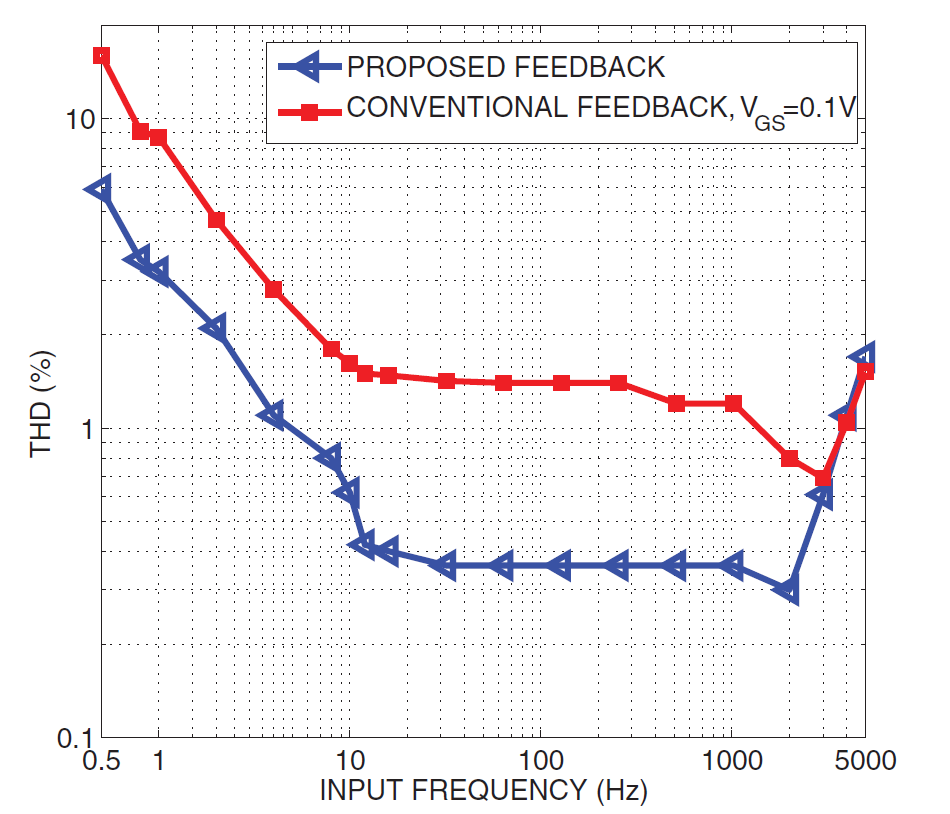
\includegraphics[scale=0.17]{Figures/genovTHD.png}
        \end{figure}
    \column{.35\textwidth}
        {\renewcommand\normalsize{\scriptsize}%
        \normalsize
            Jedyna praca, jaką udało mi się zależność wskazująca na problem nieliniowości w zakresie niskich częstotliwości, które są podstawową częścią rejestrowanych sygnałów.
            Symulacje THD dla sygnału sinusoidalnego o amplitudzie: $\SI{1.4}{\milli\volt_{pp}}$ -- K. Abdelhalim and R. Genov, doi: 10.1109/ISCAS.2012.6271415}
    \end{columns}

\end{frame}



    % Dziękuje za zwrócenie uwagi na brak odpowiednich przykładów uzasadniających znaczenie współczynnika THD dla niskoczęstotliwościowych składowych sygnałów w pracy. 



\begin{frame}[t]
    \begin{block}{\dk}
        \cit{
            Zastanawiający jest brak w analizach widmowych zarejestrowanych sygnałów, składowych sieci i ich harmonicznych.
            Być może zostały użyte filtry typu \high{notch}, ale nie wspomniano o tym w pracy.
        }
    \end{block}
    \begin{figure}[H]
        \centering
        \begin{subfigure}[b]{0.485\textwidth}
            \centering
            \includegraphics[scale = 0.75]{scripts/tmp/noiseGND_in.pdf}
        \end{subfigure}
        % \hfill
        \begin{subfigure}[b]{0.485\textwidth}
            \centering
            \includegraphics[scale = 0.75]{scripts/tmp/noiseElektrodaNaCl.pdf}
        \end{subfigure}     
    \end{figure}
\end{frame}

%%% Buchner

\begin{frame}[t]
    \begin{block}{\tb}
        \cit{
            Język rozprawy jest bardzo dobry, odnotowano jedynie nieliczne przypadki łączenia imiesłowu przysłówkowego ze stroną bierną.
        }
    \end{block}

    \begin{block}{\tb}
        \cit{
            Nie jest zachowany klasyczny układ publikacji naukowej, natomiast zaproponowany układ jest logiczny i przejrzysty.
        }
    \end{block}

    Dziękuje za uwagi dotyczące układu  pracy. Cieszę się, że zaproponowany  układ został uznany za logiczny i przejrzysty. 
    \begin{block}{\tb}
        \cit{
            Użycie bibliografii jest nieco utrudnione przez brak sortowania alfabetycznego.
        }
    \end{block}
    {\renewcommand\normalsize{\scriptsize}%
    \normalsize
        Dziękuje za uwagę dotyczącą sortowania bibliografii w pracy. 
        Sortowanie numeryczne pozwoliło mi uporządkować cytowane prace w sposób, który lepiej oddawał kolejność występowania źródeł. 
        Rozumiem, że różni czytelnicy preferują różne metody sortowania, ale w tym przypadku uznałam, że sortowanie numeryczne za bardziej odpowiednie, szczególnie że w wersji elektronicznej dzięki linkom między numerem a pozycją można łatwo odszukać interesującą pozycję w bibliografii.
    }
\end{frame}

\begin{frame}[t]
    \begin{block}{\tb}
        \cit{
            Cytowanie na ogół jest poprawne, jedynie cztery źródła to źródła internetowe, dla których jedynym adresem publikacyjnym jest strona www. 
            Podane są one [...] bez daty dostępu, co jest błędem, jednak ich charakter nie wskazuje na ulotność, ponieważ są to w większości strony firmowe, zawierające charakterystyki produktów.
        }
    \end{block}

Faktycznie doszło do pominięcia tych informacji i nie wyświetlenia ich przy konkretnych pozycjach w bibliografii.

    \begin{block}{\tb}
        \cit{
            natomiast rysunki stanowiące autocytaty z prac, których współautorką jest Autorką nie są oznaczone jako takie.
        }
    \end{block}


    Chciałabym wyjaśnić, że te rysunki stanowią autocytaty z wcześniejszych prac, w których byłam współautorem oraz autorem głównym wszystkich grafik. Rysunki zostały dostosowane i poprawione zgodnie z potrzebami i kontekstem bieżącej pracy. W związku z tym, uznałam, że nie było konieczności oznaczania ich jako autocytaty, ponieważ zostały one zmodyfikowane w celu dostosowania do przedstawianej pracy. Rozumiem jednak, że ta kwestia może wydawać się niejasna.


\end{frame}


  
\begin{frame}[t]

    \begin{block}{\tb}
        \cit{
            Protokół badania nie jest dokładnie opisany, ale zakłada badanie odpowiedzi wywołanej na mechaniczne drażnienie wibrys u szczura, z jednoczesną rejestracją aktywności LFP w obszarze od kory mózgowej (Cx) do wnętrza mózgu (Th).
        }
    \end{block}
    Eksperyment biologiczny, który jest opisany w pracy opiera się na standardowej procedurze badania odpowiedzi neuronalnej w korze mózgowe na mechaniczne drażnienie wibrys u szczura oraz aktywności spontanicznej w wzgórzu.
 Protokół badania opisany jest w formie  wystarczającej do zrozumienia otrzymanych odpowiedzi.
 Dodatkowo procedura biologiczna nie stanowiła miejsca do testowania nowych możliwości pomiarowych wymiarze neurobiologicznym i została zaproponowana przez panią dr hab. Ewę Kublik wykonującej tego typu eksperymenty i mającej ogromne doświadczenie.
 Zaprezentowane wyniki pomiarowe w tej sekcji miały służyć zademonstrowania możliwości układu w kontekście efektywnej rejestracji sygnałów LFP i potencjałów czynnościowych.
\end{frame}

\begin{frame}[t]
    \begin{block}{\tb}
        \cit{
            Kod źródłowy skryptów wypracowanych w ramach pracy nie jest częścią rozprawy ani nie jest dostępny w publicznym repozytorium, choś publikacja kodu pomogłaby w ocenie kompetencji Autorki.
        }
    \end{block}
    W pierwszym kroku chciałabym zapytać o jaki kod źródłowy chodzi ponieważ w pracy stworzono różne narzędzia prowadzące do otrzymania zweryfikowanego układu scalonego. 
    Kody żródłowe projektu układu scalonego oraz obwodu drukowanego są niemożliwe do odczytania poza środowiskiem w którym były realizowane.
    Na potrzeby pracy były one archiwizowane w repozytorium o prywatnym dostępie co jest typowe dla tego typu prac.
    W przypadku skryptów mających na celu analizę otrzymanych wyników symulacyjnych i pomiarowych również nie zostały upublicznione, ale nie one były główną kwintesencją projektu.
    Kod żródłowy systemu akwizycji danych oparty o LabView oraz Python również nie jest dostępny w publicznym repozytorium ponieważ konsekwentnie nie upubliczniałam w otwartych repozytoriach stworzonego systemu.
    
\end{frame}
\begin{frame}[t]
    \begin{block}{\tb}
        \cit{
            w analizie stanu sztuki Autorka pomija dorobek jej macierzystego zespołu, chociaż go cytuje [...].
            W związku z tym recenzent skazany jest na domysły.
            Należy przyjąć, że istotną nowością omawianej pracy jest użycie pseudorezystorów, ponieważ ta technika nie pojawia się w tytułach wymienionych [...] powyżej pozycji dorobku.
        }
    \end{block}

Jest to całkowicie nowy projekt, i nie ma bezpośredniego odniesienia do poprzednich prac zespołu dlatego nie były one szczegółowo omówione.
W poprzednich pracach zespołu zagadnienie pseudo-rezystorów nie było adresowane w żaden sposób.
Dodatkowo opracowany wzmacniacz wykonany jest w innej technologii niż dotychczasowe projekty.
Został od początku do końca opracowany i zoptymalizowany w ramach przedstawianej pracy.
Wymagało to oczywiście stworzenia indywidualnych narzędzi symulacyjnych, projektowych oraz weryfikacyjnych. 

\end{frame}


\begin{frame}[t]
    \begin{block}{\tb}
        \cit{
            Metodykę procesu badawczego należy podzielić na dwa etapy [...]. 
            Pierwszy z tych etapów nie budzi zasadniczych wątpliwości. 
            Jedyny zidentyfikowany brak dotyczy wspomnianych na str. 68 wolnozmiennych oscylacji, które nie zostały uwzględnione w scenariuszach testowych, a jak wspomniano wcześniej w tekście, mają istotne znacznie dla działalności wzmancniacza.
        }
    \end{block}
    Ze względu na złożoność czasową procedury pomiarowej (kilkaset okresów dla danej częstotliwości sygnału wejściowego) nie było możliwe przeprowadzenie dogłębnej analizy wolnozmiennych sygnałów przy ustawieniu bardzo niskiej częstotliwości granicznej dlatego oparto się w rozważaniach na pomiarach THD w funkcji częstotliwości sygnału wejściowego z ustawieniami częstotliwość granicznej powyżej 1 Hz.
    
    \begin{columns}

        \column{.43\textwidth}
        \begin{figure}[H]
            \centering
            \includegraphics[scale = 0.4]{scripts/embc2021THD_fc/embc2021THD_fc.pdf}  
        \end{figure}
    
        \column{.55\textwidth}
        Czas wykonania pomiarów przedstawionych na wykresie zajmował około tydzień roboczy. Pomiar w niższym zakresie wymagałby wielokrotnie więcej czasu. 
    \end{columns}


    % \begin{block}{\tb}
    %     \cit{
    %         Uwaga co do modelowania, wynikająca z rozważań na str. 60 jest taka, że konsekwencją zależności $C_{gb}$ od $V_{gb}$ jest obecność wyrazu kwadratowego w zależności $I_{gb}(U_{gb})$ -- warto rozważyć cząstkową publikację tego wyniku.
    %     }
    % \end{block}
    % Dziękuję za tą uwagę




\end{frame}
\begin{frame}[t]
    \begin{block}{\tb}
        \cit{
            W tekście cytowanych jest kilka rodzin modeli symulacyjnych tranzystora MOS, należy się domyślać, że w dalszym ciągu użyty został model EKV.
        }
    \end{block}

    \cit{
    Należy przypomnieć, że tworząc symulacje dostosowane do submikronowych procesów technologicznych CMOS nadal opiera się na niedoskonałych modelach BSIM w wersji 4.3.0.}

    Model EKV nie jest zaimplementowany dla modeli tranzystorów w  środowisku CADENCE, czyli narzędziach które służą przeprowadzaniu symulacji submikronowych procesów technologicznych CMOS ale jest pożyteczny w kontekście zrozumienia zjawisk fizycznych w tranzystorach MOS. 
\end{frame}

\begin{frame}[t]
    \begin{block}{\tb}

        \cit{
            {\renewcommand\normalsize{\small}%
            \normalsize
            Pewne wątpliwości budzi natomiast metodyka procesu weryfikacji w eksperymencie neurofizjologicznym.
            W przypadku pomiarów o charakterze unikatowym nie ma możliwości porównania wyniku z urządzeniami referencyjnymi.
            Wydaje się jednak, że ten przypadek tu nie zachodzi.
            Bardziej właściwe wydaje się porównanie omawianego urządzenia pomiarowego z urządzeniem referencyjnym w sposób, który wykaże prawidłowość realizowanych za jego pomocą pomiarów.
            Istnieją również wspierające ten proces metody statystyczne, takie jak metoda Blanda-Altmana.}
        }

        \cit{
            {\renewcommand\normalsize{\small}%
            \normalsize
            W przypadku niniejszej pracy zastosowano jakościową metodę weryfikacji, którą jest zgodność otrzymanych z użyciem urządzenia wyników z oczekiwaniami eksperymentatora.
            Oczekiwania te zbudowane są na podstawie dostępnej wiedzy, a ta zawiera oczywiście wyniki pomiarów, które można uznać za referencyjne.
            Jednak nie ulega wątpliwości, że tego typu analiza jest dużo słabsza z perspektywy matematycznej niż analiza porównawcza dwóch urządzeń korzystających z tego samego źródła sygnału.
        }
}
    \end{block}
    {\renewcommand\normalsize{\small}%
    \normalsize
    Eksperyment przeprowadzony w IBD był standardową procedurą opartą na doświadczeniu osoby go wykonującej, wykorzystującej różne systemy pomiarowe dlatego w momencie opisu pracy uznano za wystarczające tego typu porównanie. Dziękuję jednak za podanie propozycji w jaki sposób można byłoby udoskonalić ten aspekt co może się przydać podczas potencjalnej publikacji wyników układu scalonego.}
\end{frame}





\begin{frame}[t]
    \begin{block}{\tb}
        \cit{
            wykres przedstawiony na rys. 2.4 przedstawia filtr górnoprzepustowy a nie dolnoprzepustowy (wysoka impedancja występuje w paśmie niskich częstotliwości, a impedancja w paśmie wysokich częstości jest niska).
        }
    \end{block}

    \begin{columns}

        \column{.43\textwidth}
        \vspace{-1em}
        \begin{figure}[H]
            \includegraphics[scale = 0.5]{ch2/ImpedancjaWykres.pdf}
        \end{figure}
        \vspace{-1em}
        \begin{figure}[H]
            \includegraphics[scale = 0.2]{ch2/chemNeuroInterface.png}
        \end{figure}
    
        \column{.55\textwidth}
Wykres przedstawia charakter impedancji w zależności od częstotliwości a nie filtr.

\cit{Zależność impedancji elektrody $Z$ od częstości sygnału. 
Przy niskich częstościach element pojemnościowy $Z_{CPA}(j\omega)$ zachowuje się jak przerwa w obwodzie. 
Natomiast dla wysokich częstotliwości, element ten stanowi zwarcie w obwodzie i impedancja elektrody zmierza do $R_{SP}$. 
Dla częstości pośrednich obserwuje się nachylenie charakterystyki zależne od parametru $\beta$.}
        
    \end{columns}
\end{frame}



\begin{frame}[t]
    \vspace{-1em}
    \begin{block}{\tb}
        \cit{
            {\renewcommand\normalsize{\scriptsize}%
            \normalsize
            Autorka opisuje proces inżynierski z perspektywy ex post. 
            W związku z tym zdarza się, że relacjonując wykonane badanie czy analizę nie umieszcza na końcu rozdziału wniosków z tego badania.
            Pojawiają się one niejako mimochodem jako uzasadnienie decyzji projektowej, której podjęcie jest ralaconowane w rozdziale następnym.
            Taka sytuacja występuje na granicy rozdziałów 3.2.1 i 3.2.2, kiedy zostaje w zasadzie podjęta decyzja o eliminacji z dalszych rozważań konfiguracji variable-$V_{gs}$, do czego przesłanki dostarcza rozdział 3.2.1.
            Co do rozdziału 3.2.1 to skądinąd nie jest od początku jasne w jakim celu są prowadzone opisywane w nim rozważania.
            Staje się to jasne w rozdziale 3.2.2, kiedy okazuje się, że celem tego rozdziału było rozważenie przesłanek za wyborem jednej z dwóch konfiguracji.}
        }

        \cit{
            {\renewcommand\normalsize{\scriptsize}%
            \normalsize
            Zdarza się również, że Autorka uznaje, że wniosek w sposób oczywisty wynika z przedstawionych wykresów, co nie jest oczywiste w interdyscyplinarnym środowisku odbiorców.
            Taka sytuacja występuje na granicy rozdziałów 3.3 oraz 3.4.
            Wniosek z rysunku 3.12, który kończy analizę z rozdziału 3.3 jest podsumowany w pierwszym akapicie rozdziału 3.4.
            Takich sytuacji jest więcej, ale nie spotkałem się z oczywistą luką i brakiem informacji, a co najwyżej z jej nieodpowiednią lokalizacją.}
        }
    \end{block}
    {\renewcommand\normalsize{\small}%
    \normalsize
    W tym momencie nie jestem już w stanie niestety poprawić tekstu, ale rozumiem uwagi, że całość mogła przysporzyć trudność podczas czytania.
    W pracy opisywane są wyniki, które doprowadziły do uzyskania zamierzonego celu chociaż po drodze były różne koncepcje na temat tego jak rozwiązać problem. Zapewne to mogło również wpłynąć na to, że opisując w ten spoób procesz niektóre fragmenty są mniej zrozumiałe i lokalizacja wytłumaczenia może budzić pewne wątpliwości.}
\end{frame}


\begin{frame}[t]

    \begin{block}{\tb}
        \cit{
            Kilkukrotnie Autorka traktuje uzyskane wyniki jako oczywiste i nie tłumaczy która z cech wykresu dowodzi wyciąganego wniosku.
            W kilku przypadkach cechą tą jest różnica nachyleń między dwoma połówkami wykresy -- sytuacja ta dotyczy rys 3.11 oraz 5.18.
        }
    \end{block}
    \begin{columns}
        \column{.4\textwidth}
        Na powyższych wykresach nie ma widocznych znacznych różnic w nachyleniu wykresów, różnice wynikają z przesunięciu częstotliwości granicznych co zostało omówione w pracy wraz z powodem dla których dane zjawisko występuje. 
            \column{.3\textwidth}
            \begin{figure}[H]
                \centering
                \includegraphics[scale = 0.35]{scripts/tmp/fig3_R1.pdf}
            \end{figure}
            \column{.3\textwidth}
            \begin{figure}[H]
                \centering
                \includegraphics[scale = 0.35]{scripts/tmp/fig3_R2.pdf}
            \end{figure}
        \end{columns}
        
        \begin{figure}[H]
            \centering
            \begin{subfigure}[b]{0.485\textwidth}
                \centering
                \includegraphics[scale = 0.45]{scripts/tmp/noiseGND_in.pdf}
            \end{subfigure}
            % \hfill
            \begin{subfigure}[b]{0.485\textwidth}
                \centering
                \includegraphics[scale = 0.45]{scripts/tmp/noiseElektrodaNaCl.pdf}
            \end{subfigure}     
        \end{figure}

\end{frame}



\begin{frame}[t]
    \begin{block}{\tb}
        \cit{
            Z całkowitych drobiazgów należy zwrócić uwagę na tabelę 3.1, w której zmienna $R_f$ powinna stanowić kolejną kolumnę tabeli.
        }
    \end{block}
    % \usepackage{multirow}
% \usepackage{booktabs}
% \usepackage{hhline}

{\renewcommand\normalsize{\small}%
\normalsize

\begin{table}
    \centering
    % \caption{Wartość skuteczna szumów wejściowych dla różnych parametrów obwodu. Wartości zostały obliczane  w zakresie częstotliwości $\SI{1}{\hertz}$ -- $\SI{10}{\kilo\hertz}$.}
    % \label{table:noiseAC}
    \begin{tabular}{c||ccccc} 
    % \cmidrule[\heavyrulewidth]{1-4}\cmidrule{5-5}\cmidrule[\heavyrulewidth]{6-6}\morecmidrule\cmidrule{5-5}
    \begin{tabular}[c]{@{}c@{}}Parametry \\charakterystyczne\end{tabular}                                             & \begin{tabular}[c]{@{}c@{}}Pojemności \\sprzężenia\\~AC [F]\end{tabular} & \begin{tabular}[c]{@{}c@{}}Wzmocnienie\\~{[}V/V]\end{tabular} & \begin{tabular}[c]{@{}c@{}}Częstotliwość \\graniczna\\obwodu\\AC [Hz]\end{tabular} & \begin{tabular}[c]{@{}c@{}}Rezystancja\\$R_f$ [$\SI{}{\tera\ohm}$]\end{tabular} & \begin{tabular}[c]{@{}c@{}}Ekwiwalentne\\szumy\\wejściowe \\ {[}$\SI{}{\micro\volt_{rms}} $]\end{tabular}  \\ 
    \hhline{=::=====}
    \multirow{3}{*}{\begin{tabular}[c]{@{}c@{}}Zmienna częstotliwość \\graniczna \\(zmiana – $R_f$)\end{tabular}}     & 4 p, 200 f                                                               & 20                                                            & 1,0                                                                                & 0.79                                                         & 7,2                                                                                                        \\
                                                                                                                      & 4 p, 200 f                                                               & 20                                                            & 0,5                                                                                & 1.59                                                           & 5,5                                                                                                        \\
                                                                                                                      & 4 p, 200 f                                                               & 20                                                            & 0,2                                                                                & 3.98                                                            & 3,6                                                                                                        \\ 
    \hhline{=::=====}
    \multirow{3}{*}{\begin{tabular}[c]{@{}c@{}}Zmienne wzmocnienie\\(zmiana – $C_f$)\end{tabular}}                    & 4 p, 200 f                                                               & 20                                                            & 1,0                                                                                & 0.79                                                          & 7,2                                                                                                        \\
                                                                                                                      & 4 p, 80 f                                                                 & 50                                                            & 1,0                                                                                & 1.98                                                            & 4,6                                                                                                        \\
                                                                                                                      & 4 p, 40 f                                                                 & 100                                                           & 1,0                                                                                & 3.98                                                            & 3,2                                                                                                        \\ 
    \hhline{=::=====}
    \multirow{3}{*}{\begin{tabular}[c]{@{}c@{}}Zmienna powierzchnia \\obwodu\\(zmiana – $C_{in}$, $C_f$)\end{tabular}} & 4 p, 200 f                                                               & 20                                                            & 1,0                                                                                & 0.79                                                         & 7,2                                                                                                        \\
                                                                                                                      & 8 p, 400 f                                                               & 20                                                            & 1,0                                                                                & 0.39                                                        & 5,1                                                                                                        \\
                                                                                                                      & 12 p, 600 f                                                              & 20                                                            & 1,0                                                                                & 0.26                                                          & 4,2                                                                                                        \\
    % \cmidrule[\heavyrulewidth]{1-4}\cmidrule{5-5}\cmidrule[\heavyrulewidth]{6-6}\morecmidrule\cmidrule{5-5}
    \end{tabular}
    \end{table}

}
\end{frame}

\begin{frame}[t]

    \begin{block}{\tb}
        \cit{
            Warto również odnotować niekonsekwentny charakter opisu procesów fizykochemicznych zachodzących po stronie tkanki, które czasem opisywane są jako procesy jonowe, czasem jako procesy elektrochemiczne, a czasem odnoszone są do pojęcia warstwy podwójnej i efektów pojemnościowych.
            Co do zasady użyte modele matematyczne nie budzą wątpliwości, choć model matematyczny tkanki jest zdawkowy [...]
        }
    \end{block}
W pracy opierano się na powszechnie używanym prostym modelu tkanka elektroda. Uznano, że na potrzeby wyznaczenia celów pracy takie podejście za wystarczające. 
Praca skupiała się na aspekcie eksploracji parametrów przedwzmacniacza oraz oceny możliwości zbudowania efektywnego układu na potrzeby przyszłego systemu łączącego rejestrację i stymulacją elektryczną komórek nerwowych w mózgu na dużą skalę pomiarową.
W trakcie pisania pracy uznałam, że warto wprowadzić czytelnika w tematykę procesów zachodzących na styku elektrody i tkanki na podstawowym poziomie. 

\end{frame}

\begin{frame}[t]
    \vspace{-1em}
    \begin{block}{\tb}
        \cit{
            {\renewcommand\normalsize{\scriptsize}%
            \normalsize
            Co do mankamentów merytorycznych, występujących w dysertacji, jest ich kilka.
            Pierwszy z nich [...] dotyczy faktu, że model źródła, tkanki i sprzężenia jest niejednoznaczny i nie do końca odpowiada rzeczywistości pomiarowej.
            Niezależnie od widma samego źródła, skumulowane efekty pojemności i lokalnego przewodzenia w tkance, nakładają na źródł swoją charakterystykę, która faworyzuje niskie częstotliwości [8].
            Efekty jonowe są składową tego zjawiska [9] ale nie mają dominującego charakteru [10].}
        }

        \cit{
            {\renewcommand\normalsize{\scriptsize}%
            \normalsize
            Potencjał stały jest przede wszystki efektem brzegowym, związanym z tworzeniem warstwy podwójnej, które z kolei wynika z różnicy potencjałów chemicznych między kontaktującymi się fazami [10].
            Oczywiście rozdzielenie ładunku objętościowego również zachodzi [9], ale jest to efekt fizyczny a nie fizykochemiczny.
            Przemiany elektrochemiczne modą zachodzić dopiero gdy przekroczona jest określona energia aktywacji [10].
            W odniesieniu do elektrod stymulujących piszą o tym Merrill i wsp. -- pozycja [113] literatury -- te rozważania można rozszerzyć na elektrody pomiarowe [8-10]. }
            }

        \cit{
            {\renewcommand\normalsize{\scriptsize}%
            \normalsize
            Fluktuacje termincze dotyczą nie tylko rezystancji ale również pojemności -- taki proces jak tworzenie warstwy podwójnej również jest poddany fluktuacjom.
            W związku z tym nie ma potrzeby odwoływania się do rezystancyjnej natury tkanki, po to, żeby uzasadnić użycie twierdzenia Nyquista.
            Należy to raczej uznać za brak modelu.
            Również rezystywny charakter tkanki nerwowej można poddać w wątpliwość -- cytowany przez Autorkę Destexhe ma w swoim dorobku pracę [7] poświęconą temu zagadnieniu.
         }}
    \end{block}
\end{frame}

\begin{frame}[t]
W pracy podczas wyznaczania wymagań dla systemu ze względu na charakter sygnałów opierano się na wiedzy literaturowej osób rejestrującej takie sygnały.

Dodatkowo zakładano że w przypadku mikroelektrod umiejscowionych w bezpośrednim sąsiedztwie komórki nerwowej główny dominujący wpływ ma rezystywny charakter medium. Rejestracja w takich systemach odbywa się na bardzo krótkich dystansach.
W pomiarach EEG i Ecog sygnał transmitowany jest przez różne tkanki i zagadnienie modelowania tych sygnałów nie jest trywialne i istotne w kontekście stworzenia wiernych systemów rejestrujących.

Chciałabym podkreślić, że mimo takiego uproszczonego podejścia możliwe było wyznaczenie wymagań projektowych w kontekście szumów, zakresu amplitudy i częstotliwości rejestrowanego sygnału.

Dodatkowo głównym aspektem poruszanym w pracy była eksploracja ograniczeń technologii w kontekście stworzenia przyszłego systemu tysiące kanałów odczytowych.




\end{frame}
\begin{frame}[t]
    \begin{block}{\tb}
        \cit{
            Czynnikiem, który w sposób zasadniczy wpływa na model błędu i model sprzężenia tkanki z elektrodą jest lokalizacja elektrody referencyjnej.
            Nie ulega wątpliwości, że sonda MEA jest czymś zupełnie innym niż elektroda referencyjna, więc pomiar jest asymetryczny.
            Nie zmienia to jednak faktu, że nadal jest to pomiar bipolarny.
            Niektóre konstrukcje, takie jak opisywany przez Autorkę Neuropixel, są bipolarne i symetryczne (por rys. 2.8, także rys. 2.13) inne nie są (rys. 2.12, 3.7!).
            Zdecydowanie brakuje odniesienia do tej fundamentalnej różnicy.
            Im dalej umieszczona jest elektroda referencyjna tym większy wpływ na sygnał ma interferencja 50 Hz, oraz wszystkie źródła endogenne, w szczególności silny sygnał kardiogenny.
            Przy odległej lokalizacji elektrody odniesienia trudno jest interpretować otrzymane przebiegi jako neurogenne.
        }
    \end{block}
    
    W praktyce trudno jest zapewnić idealnie symetryczny pomiar, ponieważ impedancja elektrody referencyjne jest zawsze inna niż elektrody pomiarowej, nawet w przypadku sondy Neuropixel. Możliwym rozwiązaniem, stosowanym zresztą powszechnie, jest wykonanie elektrody referencyjnej o możliwie małej impedancji. Oczywiście nie zapewnia to tłumienia sygnałów współbieżnych generowanych w badanej tkance, ale pomaga w tłumieniu sygnałów współbieżnych pochodzących z zakłóceń elektromagnetycznych. 
\end{frame}



\begin{frame}[t]
    \begin{columns}

    \column{.475\textwidth}
\begin{figure}[H]
    \centering
    \includegraphics[scale=0.1]{ch2/neuropixelsch.png} 
    \includegraphics[scale=0.5]{ch2/conceptAC_Harrison.pdf} 

\end{figure}

\column{.475\textwidth}
\begin{figure}[H]
    \centering
    \includegraphics[scale=0.3]{ch2/crosstalkSch.jpg} 
    \includegraphics[scale=0.5]{ch3/pseudo-lay.pdf} 


\end{figure}
\end{columns}
\end{frame}

\begin{frame}[t]
    \vspace{-1em}
    \begin{block}{\tb}
        \cit{
            Odwrócenie amplitudy obserwowane na elektrodzie 0 wygląda w pierwszym przybliżeniu na wynik zmiany fazy wynikający ze sprzężenia pojemnościowego -- trudno byłoby zinterpretować odwrócenie amplitudy wprost jako odwrócenie kierunku prądu -- jest to jeden z najciekawszych wyników dotyczących samych narzędzi, sugerujący konieczność dalszego rozwoju techniki modelowania.
        }
    \end{block}

    \begin{columns}

        \column{.2\textwidth}
\vspace{-1em}
        \begin{figure}
            \centering
            \includegraphics[scale=0.3]{scripts/tmp/avgLFPResponseMap_filtering39.pdf}
        \end{figure}
        \column{.78\textwidth}
        {\renewcommand\normalsize{\small}%
        \normalsize
        \cit{Polarność sygnału wskazuje na kierunek przepływu jonów, do elektrody lub od elektrody.} - ten fragment tyczy się wytłumaczenia tego dlaczego poszczególne panele się różną, nie odnoszą się do tego co się stało na elektrodzie zero. Zgodnie z wiedzą ekspercką osoby wykonującej pomiar i jej doświadczeniem w poprzednich eksperymentach efekt na elektrodzie zerowej został wytłumaczony jak efekt pracy tkanki i obserwowane sygnały.
        W pracy przedstawiono to wytłumaczenie jednak niestety w niezbyt klarowny sposób.

        \cit{Jeżeli uwzględnimy fakt, że pokazane dwie serie rejestracji zostały wykonane w znacznym odstępie czasowym ok. 100 minut, obserwację zmiany kształtu sygnały z bipolarnego na unipolarny należy interpretować jako zmianę w strukturze tkanki w pobliżu danej elektrody. 
        Warstwa powierzchniowa tkanki jest bardziej narażana na wpływ czynników zewnętrznych, natomiast głębsze warstwy kory baryłkowej pozostają bardziej stabilne w czasie, co potwierdzają zarejestrowane sygnały.}}

    \end{columns}
\end{frame}

\begin{frame}[t]
    \vspace{-1em}
    \begin{block}{\tb}
        \cit{
            Odnośnie podnoszonego przez Autorkę faktu zniknięcia podwójnego maksimum widma THD, warto zauważyć, że rozwiązanie takie występowało już jako jeden z wariantów widma w analizie Monte-Carlo (rys 4.9) oraz wykazywało silną zależność od pojemności $C_{gb}$ (rys 3.10), co mogło być przyczyną obserwowanych różnic między widmem zmierzonym a wynikami symulacji.
        }
    \end{block}
W pracy nie ma analitycznego wytłumaczenia charakteru zmian kształtu krzywej THD, ale należy przyjąć, że bardziej wiarygodny jest wynik otrzymany w pomiarach ponieważ środowisko symulacyjne może nie uwzględniać wszystkich efektów technologii jeżeli stosuje sią ją w dosyć nietypowych wariantach (brzegowych parametrach).  
\vspace{-2em}

    \begin{columns}

        \column{.3\textwidth}
    \begin{figure}[H]
    \centering
    \includegraphics[scale = 0.5]{scripts/analyseTran/analyseTranTechnology.pdf}
    \end{figure}
        
    \column{.3\textwidth}

    \begin{figure}[H]
        \centering
    \includegraphics[scale = 0.5]{scripts/mcTranResult/mcTranResult.pdf}
    \end{figure}

    \column{.3\textwidth}
    \begin{figure}[H]
        \centering
        \includegraphics[trim={0 0.25cm 0 0.25cm}, clip, scale = 0.5]{scripts/embc2021THD_size/embc2021THD_size_0_100.pdf}
    \end{figure}
        


    \end{columns}
\end{frame}

% \begin{frame}[t]
%     \begin{block}{\tb}
%         \cit{

%         }
%     \end{block}
% \end{frame}

